\documentclass[a4paper,11pt]{article}
\usepackage[utf8]{inputenc}
\usepackage{lmodern}
\usepackage{amsmath}
\usepackage{enumitem}
\usepackage{graphicx}
\title{\Huge Modelo de Predicción de Demanda y Pricing Dinámico}
\author{Oscar Daniel Camarena Gómez}
\date{}
\begin{document}
\maketitle
\pagenumbering{gobble}
\newpage
\pagenumbering{arabic}
\section{Introducción}
\paragraph {CityExpress} ~ \\
CityExpress es una cadena de hoteles 100\% mexicana enfocada al turismo de negocios. Actualmente cuenta con 140 hoteles en México y Latinoamérica (Colombia, Costa Rica y Chile). CityExpress cuenta con hoteles pensados para el viajero de negocios, sus instalaciones son prácticas, la tarifa es baja y ofrece servicios limitados pero valiosos durante un viaje de negocios, por ejemplo:
\begin{itemize}[noitemsep]
\item Internet gratuito en las habitaciones
\item Desayuno de cortesía
\item Transporte gratuito 10 km a la redonda
\item Servicio estandarizado con bajo costo
\end{itemize}
CityExpress cuenta con 4 marcas, cada una de ellas enfocada a distintos segmentos de mercado:
\begin{description}
\item [$\bullet$ CityExpress:] Marca emblema, enfocada al viajero de negocios. Los hoteles están ubicados cerca de los centros de negocios de las distintas ciudades en la República Mexicana.
\item [$\bullet$ CityExpress Plus:] Hoteles ubicados en las principales ciudades de la República Mexicana (CDMX, Guadalajara, Monterrey) y en Latinoamérica (Colombia). Ofrecen diseños vanguardistas y mayor espacio en las habitaciones.
\item [$\bullet$ CityExpress Suites:] Marca enfocada en los viajeros de larga estancia. Sus instalaciones cuentan con cocineta, estancia y habitaciones de mayor tamaño.
\item [$\bullet$ CityExpress Junior:] Hoteles de menor precio enfocados al turismo con presupuesto limitado ofreciendo un producto de calidad y con servicio estandarizado.
\end{description}
\paragraph {Ubicación} ~ \\
Típicamente un hotel de CityExpress está ubicado cerca de zonas industriales o zonas con fuerte actividad económica, es decir, en el caso de las grandes ciudades encontraremos hoteles CityExpress cerca de una zona donde hay alta densidad de locales comerciales, oficinas corporativas o centros de negocios. En el caso de ciudades mas pequeñas o con actividades económicas específicas encontraremos hoteles cerca de los centros económicos de cada una de las ciudades, este hecho permite que la cadena agrupe a sus hoteles en distintos \textbf{corredores} dependiendo de la actividad de las zonas económicas donde se encuentran. A continuación se presentan los distintos corredores:
\begin{itemize}[noitemsep]
\item Energético
\item Exportacion-Agricultura
\item Franquicia
\item Internacional
\item Manufactura
\item Maquila
\item Mineria
\item Servicios
\end{itemize}
\paragraph {Hoteles} ~ \\
Las propiedades de Hoteles CityExpress siguen un estándar desde su construcción hasta en su operación diaria. En cuanto al estándar de construcción las propiedades generalmente cuentan con 6 plantas, 120 habitaciones, un lobby para la recepción de huéspedes y áreas comunes; por ejemplo, área designada para fumar, desayunador, salas de juntas, salones de eventos y alberca (en algunas propiedades). 
En cuanto a las habitaciones el tamaño puede variar por marca, sin embargo ofrecen los mismos servicios independientemente de ella: 
\begin{itemize}[noitemsep]
\item Internet Gratuito
\item Área de Trabajo
\item Lavandería
\item Aire Acondicionado
\item Pantalla de televisión
\item Desayuno de cortesía
\end{itemize}
\paragraph {Crecimiento} ~ \\
Hoteles CityExpress fue fundada en 2002 con su primer hotel construido en Saltillo. A partir de ese entonces se ejecutó un ambicioso plan de crecimiento en el cuál se impuso la meta de abrir un nuevo hotel cada 6.8 semanas. Esto llevo a que la cadena de hoteles contara con más de 140 propiedades en un lapso de 16 años.
Hoy en día Hoteles CityExpress cuenta con propiedades en 34 de los 36 estados de la República Mexicana y 5 mas en Latinoamérica: 1 en Costa Rica, 1 en Chile, 3 en Colombia. El plan de crecimiento sigue siendo ambicioso y la cadena espera contar con 180 propiedades para el 2020.
\begin{figure}[!]
  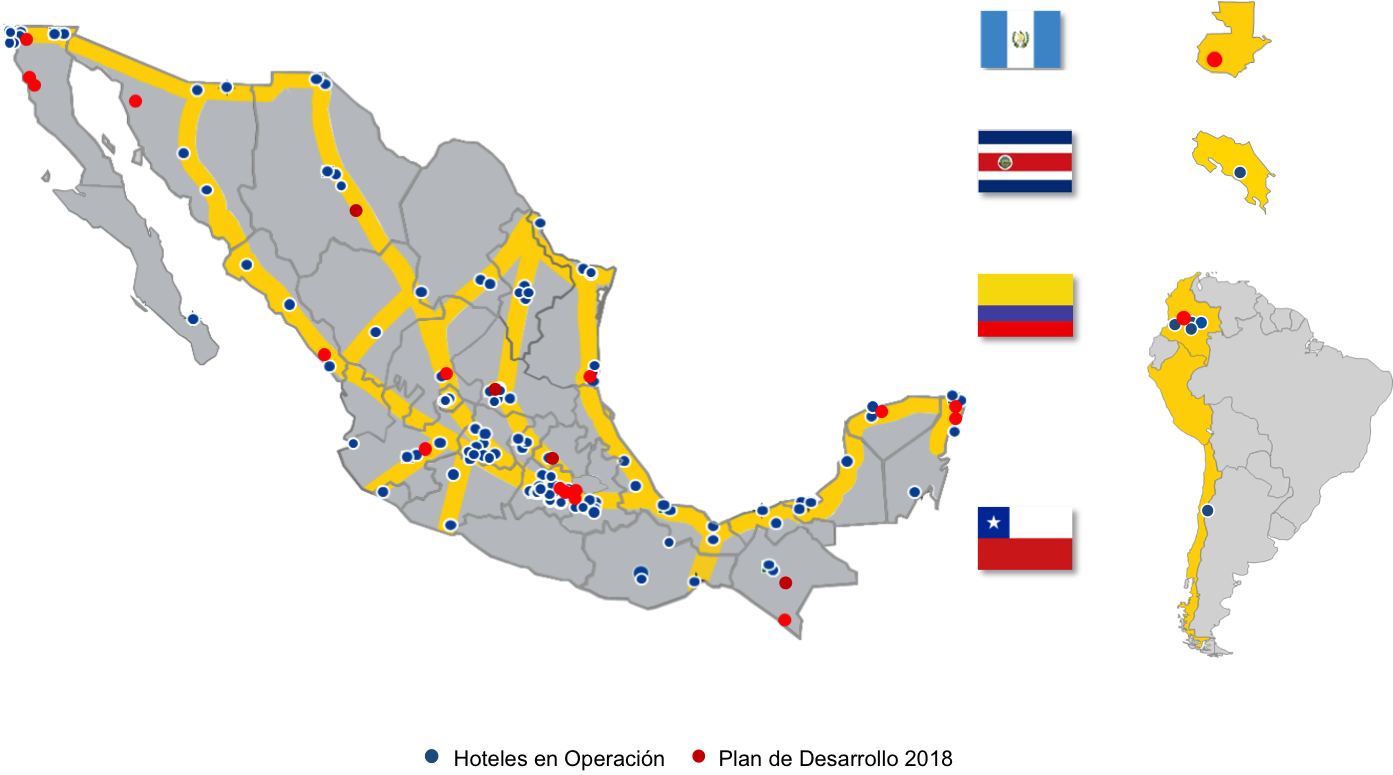
\includegraphics[width=\linewidth]{Imagenes/Ubicaciones.png}
  \caption{Plan de crecimiento}
  \label{fig:crecimiento}
\end{figure}
\section{Descripción del Problema}
\subsection{Gestión de las propiedades}
Hoteles CityExpress cuenta con un modelo de gestión comercial de sus propiedades ejecutado desde sus oficinas centrales ubicadas en la Ciudad de México. Este modelo de gestión se enfoca en optimizar la venta de los cuartos de las distintas propiedades, buscando siempre maximizar el ingreso obtenido por estas ventas.
Para poder entender mejor el modelo de gestión comercial debemos estudiar antes los canales distribución que utiliza para la venta de sus productos así como sus distintos segmentos de mercado. Posteriormente presentaremos las principales variables utilizadas para calificar el desempeño de las propiedades así como las acciones que puede tomar cada uno de los gerentes de las propiedades para poder cambiar el desempeño del hotel.
\paragraph{Canales de Venta} ~\\
CityExpress cuenta con un modelo de venta estandarizado para todas sus propiedades. Este modelo de venta contempla distintos canales de distribución que ayudan al grupo a poder incrementar la oferta de su producto llegando a distintos segmentos de mercado.
Es importante mencionar que cada uno de los canales de venta tienen un costo asociado, es decir, del ingreso que se perciba por cada cuarto vendido se debe tomar en cuenta el costo de cada canal para poder calcular la utilidad bruta de la venta, por eso es. importante conocer cómo opera cada uno de ellos.
Dentro de CityExpress existen dos tipos de canales de venta: \textbf{Canales de venta tradicionales} y \textbf{Canales de venta electrónicos}. Los canales de venta tradicionales, son aquellos en los cuales se requiere la intervención de un agente de ventas, los electrónicos permiten que el cliente final realice su reservación sin requerir la intervención del agente:
\paragraph{\textbf{Canales de venta tradicionales}}
\begin{itemize}[noitemsep]
\item Centro de Contacto (Call Center)
\item Hotel
\end{itemize}
\paragraph{\textbf{Canales de venta electrónicos}}
\begin{itemize}[noitemsep]
\item App (IOS y Android)
\item Portal Cliente Frecuente (City Premios)
\item Motor de reservaciones corporativas (CityAccess)
\item Motor de reservaciones (www.cityexpress.com.mx)
\item Agencias de viajes en línea (OTAs)
\end{itemize}
\paragraph{Segmentos de Mercado} ~\\
Los segmentos de mercado son un punto medular para poder entender el modelo de gestión en CityExpress ya que estos permiten al área comercial poder establecer una estrategia de venta en cada uno de los canales fijando precios en las distintas tarifas para poder maximizar la ocupación del hotel y el ingreso por cuartos vendidos. 
Típicamente un hotel cuenta con un conjunto de tarifas las cuales son ofrecidas a diferentes segmentos de mercado en diferentes canales. Por ejemplo, un huésped que viaja por placer y reserva por la página web de CityExpress muy probablemente recibirá una tarifa distinta al huésped que viaja por negocios y reservó por el centro de contacto.
A continuación se presentan los distintos segmentos de mercado manejados por CityExpress:
\paragraph{\textbf{Negocios}}
\begin{itemize}[noitemsep]
\item Directos
\item Convenios
\item Viajero Frecuente
\item Corporativo
\item Consorcios
\item Promociones
\item Otros
\end{itemize}
\paragraph{\textbf{Placer}}
\begin{itemize}[noitemsep]
\item Directos
\item Fin de Semana
\item Otros
\item Promociones
\end{itemize}
\paragraph{\textbf{Mayoreo}}
\begin{itemize}[noitemsep]
\item Agencias Minoristas
\item OTAs
\item Lineas Aéreas / Tripulaciones
\item Agencias Mayoristas
\item Otros
\end{itemize}
\paragraph{\textbf{Grupos}}
\begin{itemize}[noitemsep]
\item Grupos, Ferias, Congresos y Convenciones
\item Sociales
\item Juntas
\item Deportes
\end{itemize}
\paragraph{\textbf{Otros}}
\begin{itemize}[noitemsep]
\item Uso Casa
\item Cortesías
\item Intercambio
\item Empleados
\item Industria Turística
\item Otros
\end{itemize}
\paragraph{Tarifas} ~\\
Como se mencionó anteriormente, un hotel tiene un catálogo de 36 tarifas que puede ofrecer a los huéspedes. Cada tarifa va dirigida a un segmento de mercado y un canal en específico. Hay tarifas que pueden cambiar de precio hasta 3 veces al día y hay otras que al ser tarifas convenidas con otras empresas, permanecen estáticas la mayor parte del año.
Es responsabilidad de cada uno de los hoteles el revisar los distintos reportes expuestos en la organización en donde pueden encontrar: sus niveles de ocupación, ocupación de la competencia, tarifas promedio propias, tarifas promedio de la competencia, penetración de ocupación: $\frac{\% ocupacion\ propia}{ \% ocupacion\ de\ la\ competencia}$ y penetración de tarifa: $\frac{tarifa\ promedio\ propia}{tarifa\ promedio\ de\ la\ competencia}$ para decidir si deben hacer un incremento o decremento en los precios ofertados.
\paragraph{Variables estudiadas} ~\\
Dentro de CityExpress las decisiones de cambios de precios en las tarifas se toma analizando distintas variables. La mayoría de estas variables se alimentan de información propia del grupo hotelero aunque hay algunas que se obtienen de información de la competencia. A continuación se detallará cada una de las variables utilizadas durante la toma de estas decisiones:
\begin{itemize}[noitemsep]
\item \%Ocupacion
\item Tarifa Promedio
\item Tarifa Efectiva
\item Penetración de Ocupación
\item Penetración de Tarifa
\item Eventos por plaza
\item \%Ocupación de la competencia
\item Tarifa Promedio de la competencia
\item Tarifa Efectiva de la competencia
\end{itemize}
Derivado de las conclusiones del análisis de estas variables, los hoteles y el equipo de la oficina central pueden tomar alguna de las siguientes decisiones para alcanzar el objetivo deseado:
\begin{itemize}[noitemsep]
\item Subir precio de tarifa
\item Bajar precio de tarifa
\item Abrir un canal de venta
\item Cerrar un canal de venta
\item Promover la venta de un segmento específico mediante una promoción
\item Inhibir la venta de un segmento en específico cerrando disponibilidad de alguna tarifa
\end{itemize}
\subsection{Situación Actual}
Como se mencionó en el apartado anterior, hoy en día CityExpress gestiona su estrategia comercial desde las oficinas centrales delegando tareas clave a cada uno de los gerentes de las distintas propiedades, esto aunado al ambicioso plan de crecimiento de la cadena ha hecho que este modelo de gestión comercial se vuelva un proceso complicado de administrar y ejecutar de manera efectiva ya que se tienen las siguientes dependencias en el proceso:
 \begin{itemize}[noitemsep]
\item Publicación de reportes diarios
\item Análisis de información publicada
\item Presentación de plan de acción de acuerdo al modelo de gestión
\item Aprobación del plan de acción por parte de la oficina central
\item Ejecución del plan de acción en los sistemas de control
\item Validación de resultados del plan de acción
\end{itemize}
\subsection{Propuesta de mejora al proceso}
Este proyecto tiene como objetivo mejorar el proceso de gestión de hoteles en CityExpress mediante la construcción de un sitio en donde se integre toda la información que hoy en día se expone en distintos reportes dentro de la empresa y además cuente con un modelo que permita pronosticar el $\%\ de\ ocupacion$ de cada una de las propiedades y a su vez haga una recomendación del precio para la tarifa que se ofrece al público en general que ayude a maximizar el ingreso por venta de cuartos dentro de la propiedad.
Con esta herramienta se espera que el modelo de gestión comercial se automatice y la ejecución del plan de acción se realice de manera más ágil.
\section{Metodología Propuesta}
\subsection{Plan de implementación}
A continuación se presentan los pasos que se siguieron para la implementación de este nuevo sistema de gestión:
\begin{description}
\item [$\bullet$ Entendimiento del negocio:]  Antes de construir una herramienta / producto de datos se dedicó un tiempo a conocer los procesos operativos de la cadena hotelera.
\item [$\bullet$ Entendimiento del sistema de gestión comercial:] Para que el producto final agregue verdadero valor a la empresa se debió comprender el tramo de control de cada puesto operativo destinado a hacer uso de esta herramienta, es decir, se identificaron las acciones que cada usuario puede ejecutar en los distintos sistemas para alcanzar sus objetivos comerciales.
\item [$\bullet$ Identificación de posibles fuentes de datos:] Una vez comprendidos los procesos operativos y de toma de decisiones, se identificaron los sistemas que proveen la información que ayuda al personal de CityExpress durante la toma de decisiones.
\item [$\bullet$ Análisis exploratorio de datos:] Una vez identificadas las fuentes de datos, se ejecutó un análisis exploratorio de datos con el fin de poder conocer los datos con que se trabajaron para posteriormente fijar un alcance para el producto final.
\item [$\bullet$ Modelo de predicción de ocupación y sugerencia de precios:] Una vez perfilados los datos y con un EDA concluido se realizó un esfuerzo para construir un modelo que fuera capaz de pronosticar el $\%\ de\ ocupacion$ y que sugiriera el $precio\ publico$ óptimo de cada una de las propiedades.
\item [$\bullet$ Construcción de prototipo de producto de datos:] Para finalizar este proyecto, se definió la arquitectura final del producto de datos y se construyó un prototipo totalmente funcional que apoya la toma de decisiones de los participantes del proceso de gestión comercial.
\end{description}
\subsection{Fuentes de datos}
\section{Resultados}
\section{Referencias}

\end{document}